\documentclass[10pt,twocolumn]{article}
\usepackage[a4paper,margin=17mm,columnsep=7mm]{geometry}
\usepackage{amsmath,amssymb,amsthm,graphicx,hyperref,microtype,balance}
\hypersetup{colorlinks=true,linkcolor=blue,urlcolor=blue,citecolor=blue}
\newtheorem{theorem}{Theorem}
\title{Convergence of the Tetrad and Collective Flywheel Geometries}
\author{Stephen Nelson \\ Field Dynamics Research}
\date{November 2026 \quad | \quad Proof 25}
\begin{document}
\twocolumn[\maketitle\begin{abstract}The preceding tetrad, Hadamard and vortex proofs describe the same regular spatial frame through different constructions. We give a common finite-dimensional formulation that makes their relationship explicit. Four simple triangular cycles with the stated pairwise incidence determine the tetrahedral graph. With the inherited Euclidean norms, the spatial frame, the oriented cycle and cut frames, and the row-closed flywheel phase read have the common Gram matrix $G=4I-J$. Their canonical partial isometries compose independently of the chosen route. A signed complementary-edge involution explains the axial versus polar distinction. Intrinsic closure coordinates recover the two bounded simplices, their octahedral intersection and eight stellations. Pair incidence gives the core metric and the face-dual cube, linking the collective current to the outer phase reads. We prove metric rigidity and sharp anisotropy bounds. These are conditional mathematical equivalences, not a derivation of physical geometry formation or gravitational dynamics from a fixed graph.
\end{abstract}\vspace{3mm}]
\section*{Setting and purpose}
The geometric construction of the spatial tetrad~\cite{frame,half,scheme,gram,hadamard} and the circulation results~\cite{vortex,flywheel,p24} meet in one normed closure space. This paper makes that convergence an explicit theorem. The reader need not infer a physical mechanism from a picture, nor regard equal dimensions as evidence of equivalent representations.

We use the four labelled records $L=\{0,1,2,3\}$, with ordinary positive Euclidean inner products unless another normalization is stated. The spatial sign frame is $M\in\mathbb R^{3\times4}$, with columns $(1,1,1),(1,-1,-1),(-1,1,-1),(-1,-1,1)$, denoted $s_i$. The matrix $J_d$ is the $d\times d$ all-ones matrix; $J=J_4$. The regular spatial realization is conditional on equal magnitudes, equal pair relations, noncoincidence and dimension three. It is not inferred from the Lorentz signature alone. The two orientation sectors of the full tetrad at fixed time orientation are not two individual solutions. We use $+$ and $-$ for the positive-vertex and inverted solids, avoiding the opposite naming conventions in the source papers.

\paragraph{What the earlier routes supply.} The forced-frame proof gives the regular Gram; the half-space proof gives boundedness and overlap; the scheme distinguishes determinant signs; the Hadamard proof gives an orthogonal completion. The vortex theorem establishes circulating states on its prescribed graphs. The sustained Stage VII model uses the specified $33$ sites and $104$ bonds, with a collective three-amplitude ansatz; Proof 24 establishes the cycle and column-frame identities for that model. The recursive refinement of Proof 23 is downstream of the spatial geometry. These routes share premises and are not independent physical measurements.

\section*{1. Recognizing the incidence}
\textit{Purpose.} Before introducing spatial coordinates, identify the connectivity implied by the circulation relations.

\begin{theorem}[Triangle recognition]\label{thm:recognition}
In a simple undirected graph, let four distinct simple $3$-cycles share exactly one undirected edge per pair, with no edge used by more than two cycles. Their edge union is $K_4$. Coherent boundary orientations exist and are unique up to common reversal.
\end{theorem}
\begin{proof}
Label one triangle $012$. The other three must share different edges with it, so they have vertex triples $01a,02b,12c$, where $a,b,c$ lie outside $012$. The first two of these share an edge only when $a=b$; comparing the first and third gives $a=c$. Thus all four triangles are exactly the four faces of the abstract tetrahedron on $0,1,2,a$. Orienting them as the boundary of an oriented simplex gives opposite directions on each shared edge. Since the face adjacency is connected, a choice on one face determines all others.
\end{proof}
Without the edge multiplicity condition, four triangles sharing one fixed edge and having four different outside vertices meet the pairwise-overlap premise but are not $K_4$. The recognized cycles are the \emph{abstract} four-leg circulation patterns; we have not proved that four physical rings share these actual bonds, nor that an unconstrained flow assembles this incidence.

\section*{2. The common normalized frame}
\textit{Purpose.} Isolate the shared metric, with its normalization and its necessary symmetry assumptions.

Put $W=\mathbf1^\perp\subset\mathbb R^4$, $P=I-J/4$ and $G=4P$. Then $P^2=P=P^T$ and $\operatorname{rank}P=3$. Call $X:\mathbb R^4\to E$ a normalized closure frame when $X^TX=G$, with $E$ finite Euclidean. In particular $X\mathbf1=0$ by taking its squared norm, so $XP=X$, and $X/2$ is an isometry on $W$.

\begin{theorem}[Common Gram]\label{thm:gram}
The following five frames satisfy $X^TX=G$: $2P$, $M$, $B^T$, $D$, and $F$. Here $B$ is the vertex-edge incidence of $K_4$, $D$ the coherent face boundary matrix, and $F=\sqrt{3/2}\,C^T$ is the row-closed flywheel column frame defined below.
\end{theorem}
\begin{proof}
For $2P$ this is idempotence. For the spatial frame it follows from $M^TM=G$, $MM^T=4I_3$. More generally, if four vectors in $\mathbb R^3$ have common squared length $c^2$, common pair product $b$, and are not all coincident, their Gram is $(c^2-b)I+bJ$. Squared pair distance gives $c^2-b>0$. Rank at most three forces $c^2+3b=0$; choosing $c^2=3$ fixes the scale. Appending a row of ones to $M$ gives $H_4$ with $H_4^TH_4=4I$. Only its spatial part is a rank-three frame.

Orient each of the six edges from the lower label to the higher. Each vertex has degree three, and two distinct vertices share one edge with opposite signs; thus $BB^T=G$. In $D$, the four oriented triangular boundaries each have squared norm three and pair product $-1$, so $D^TD=G$. Since $BD=0$ and both maps have rank three, $\operatorname{im}D=\ker B$ and
\begin{equation}
 B^TB+DD^T=4I_6.\label{eq:split}
\end{equation}
For the twelve ordered pairs $(i,j)$, $i\ne j$, let $R$ and $Q$ sum rows and columns, respectively. Then $RR^T=QQ^T=3I$, $RQ^T=J-I$. The projector onto row-closed patterns is $P_r=I-R^TR/3$. For $C=QP_r$,
\begin{equation}
 CC^T=3I-(J-I)^2/3=\tfrac23G.
\end{equation}
Hence $F^TF=G$. For $q\in W$, the unique minimum-norm row-closed preimage with $QX=q$ is $(3/8)C^Tq$; it is orthogonal to $\ker C$ inside $\ker R$. This last assertion is linear algebra, not a physical energy-minimization principle.
\end{proof}

\paragraph{The signed complementary-edge map.} In edge order $01,02,03,12,13,23$, let $S$ swap $01\leftrightarrow23$ and $03\leftrightarrow12$ with sign $-1$, and $02\leftrightarrow13$ with sign $+1$. With the oriented simplex boundary convention $(-1)^i$ for omitted label $i$,
\begin{equation}
 S^T=S,\quad S^2=I,\quad SB^T=D.\label{eq:star}
\end{equation}
These equalities follow by inserting the incidence columns. This is the negative of the four-dimensional oriented Hodge star on the edge bivectors in the chosen convention. Under a label permutation $T$, the signed edge permutation $E$ obeys $ES=\operatorname{sgn}(T)SE$, since the oriented volume changes by that sign. Hence $EB^T=B^TT$ but $ED=\operatorname{sgn}(T)DT$. The cycle frame is axial, the spatial and column frames polar. Their Euclidean isometry is not an untwisted $S_4$ intertwiner; it is untwisted for $A_4$.

\section*{3. Exact convergence of all routes}
\textit{Purpose.} A common Gram must give a unique geometric correspondence rather than merely agreeing entries.

\begin{theorem}[Canonical transport]\label{thm:transport}
For any normalized closure frames $X,Y,Z$ in possibly different finite Euclidean target spaces, define $U_{YX}=YX^T/4$ and $\Pi_X=XX^T/4$. Then
\begin{align}
 U_{YX}X&=Y,\quad U_{YX}^TU_{YX}=\Pi_X,\\
 U_{YX}U_{YX}^T&=\Pi_Y,\\
 U_{ZY}U_{YX}&=U_{ZX}.\label{eq:compose}
\end{align}
The map is the unique isometry from $\operatorname{im}X$ to $\operatorname{im}Y$ matching the labelled columns, extended by zero on the orthogonal complement.
\end{theorem}
\begin{proof}
The common Gram implies $XP=X$, as above. $\Pi_X$ is symmetric and idempotent by inserting $X^TX=4P$. Its image is $\operatorname{im}X$, since $\Pi_XX=X$. Substitution proves the first three identities. For composition,
\[
 \frac{ZY^TYX^T}{16}=\frac{ZPX^T}{4}=\frac{ZX^T}{4}.
\]
The columns span $\operatorname{im}X$, so any matching map agrees there. The projector identities prove norm preservation on that image and vanishing on its complement. Repeated composition proves path independence for arbitrary finite chains.
\end{proof}
This supplies the new convergence statement. A closed chain returns the identity \emph{on the frame image}, not on its entire ambient space. These algebraic coordinate changes are not physical spacetime holonomy. The sign twist in (\ref{eq:star}) remains part of the orientation dictionary.

\section*{4. Reconstructing the two solids}
\textit{Purpose.} The correspondence should recover the entire stellated octahedron, not just four directions.

\begin{theorem}[Intrinsic dual geometry]\label{thm:solid}
Equip $W$ with inner product $q^Tr/4$. Set $a_i=Ge_i$ and $S_\pm=\operatorname{conv}\{\pm a_i\}$. Then
\begin{align}
 S_+&=\{q\in W:q_i\geq-1\},\\
 S_-&=\{q\in W:q_i\leq1\},\\
 \mathcal O=S_+\cap S_-&=W\cap[-1,1]^4.
\end{align}
Only the two uniform choices among the sixteen inequalities are bounded. $\mathcal O$ has six vertices, the permutations of $(1,1,-1,-1)$, and each $S_\pm\setminus\mathcal O$ has four stellation regions. The map $q\mapsto Mq/4$ realizes these as the regular dual tetrahedra and octahedron in space.
\end{theorem}
\begin{proof}
Since $q=M^Tx$ and $MM^T=4I_3$, the inverse $Mq/4$ preserves the stated norm. The barycentric coordinates in $S_+$ are $\lambda_i=(q_i+1)/4$; they sum to one and $G\lambda=q$. Inversion gives $S_-$. The uniform inequalities are bounded by the zero-sum relation. For a mixed choice, let $U,L$ be the nonempty upper and lower sets. The nonzero zero-sum vector $d_i=-|L|$ on $U$ and $d_i=|U|$ on $L$ defines the unbounded ray $td$, $t\geq0$.

If two coordinates of a point in $\mathcal O$ are unsaturated, opposite perturbations make it a nontrivial midpoint. Three saturated coordinates force the fourth to be saturated by the sum and the bound. Conversely a fully saturated point is extreme. The six possibilities are $(a_i+a_j)/2$, and map to the six signed coordinate axes. A point of $S_+\setminus\mathcal O$ has exactly one $q_i>1$, or $\lambda_i>1/2$. The closure of that region is the simplex with $\lambda=(e_i+\eta)/2$ for $\eta$ in the standard simplex. Its vertices are $a_i$ and the three adjacent midpoints. Inversion gives the other four. Their interiors are disjoint.
\end{proof}
The scheme's equation $(\det e)^2=\det g/\det\eta$ fixes the determinant magnitude, not an individual tetrad. At fixed observer and time orientation spatial parity exchanges the two signs and acts here by $q\mapsto-q$. The Gram is blind to the common sign. The determinant equation alone does not produce the regular spatial frame. Thus the two routes converge after the specified spatial realization, not before it.

\section*{5. The core and collective circulation}
\textit{Purpose.} Recover the central structure and the edge-current law from the same four labels.

\begin{theorem}[Pair-incidence core]\label{thm:core}
Let $N$ be the unsigned vertex-pair incidence matrix of $K_4$, $A$ the adjacency of its line graph, and $V=MN/2$. Then
\begin{equation}
 V^TV=2I_6+A-J_6,\qquad VV^T=2I_3.
\end{equation}
The core face-dual graph is $K_{4,4}$ minus a matching. Its divergence-free current space splits under chamber inversion into dimensions $3+2$; the collective Stage VII current belongs to the three-dimensional even part.
\end{theorem}
\begin{proof}
$N^TN=2I_6+A$, $NN^T=2I_4+J$ and $N^TJN=4J_6$ by incidence. Substitute $M^TM=G$ and $M\mathbf1=0$. Thus the core vertices have unit length, pair product zero if their labels share one index, and $-1$ for disjoint pairs: three antipodal orthogonal pairs. The eight triangular faces are the stars containing $i$ and triangles avoiding $j$, the facets $q_i=1$ and $q_j=-1$. Opposite families meet along an edge iff $i\ne j$; same-family faces share at most a vertex. Hence the dual graph is the connected cube, with $8$ nodes and $12$ edges. The shared primal edge corresponding to dual edge $(i,j)$ has midpoint $(a_i-a_j)/4$. Chamber inversion exchanges $(i,j)$ and $(j,i)$.

Orient currents from the positive to negative family. Divergence-free off-diagonal arrays $I$ have zero row and column sums, and dimension $12-8+1=5$. Inversion acts as $I\mapsto-I^T$. The antisymmetric part identifies with $\ker B$, dimension three. The symmetric part has six free entries and four independent row constraints: a relation among the constraints requires $c_i+c_j=0$ for every pair, which forces all $c_i=0$ using a triangle. This gives the two odd dimensions.

For collective phase $q=x+iy\in W_{\mathbb C}$, let $a_{ij}=x_i y_j-y_i x_j$. Row sums vanish, so $a\in\ker B$ in oriented six-edge coordinates. Every bivector of the three-space $W$ is decomposable, and $\Lambda^2W$ maps injectively into the three-dimensional antisymmetric cycle space; thus this wedge describes all its directions. For $j_0=D^Ta$, (\ref{eq:split}) implies $Dj_0=4a$. In the inherited Stage VII model with $r=k=-1$, scale $\rho$ and amplitudes $v,w$, Proof 24 gives the consistently oriented means $j=(2\rho^2|v|^2/3)D^Ta$ and independent core currents $I_e=2\rho^2|w|^2a$. Therefore
\begin{equation}
 |v|^2 I_e=\tfrac34|w|^2 Dj.\label{eq:current}
\end{equation}
The equality also holds at zero winding. The remaining six core entries follow by antisymmetry.
\end{proof}
Equation (\ref{eq:current}) uses the existing common phase, not an independent core oscillator. The eight physical outer rings are not the four abstract triangular cycles of Theorem~\ref{thm:recognition}; the phase and current dictionary is what links them. A particular circulating solution does not occupy every direction of the available current space. No axial through-flow is implied by these closed currents.

\section*{6. Rigidity and sharp metric dependence}
\textit{Purpose.} State exactly which hypotheses matter, and quantify failure when they are relaxed.

\begin{theorem}[Diagonal metric rigidity]\label{thm:rigidity}
For positive edge weights $w_e$, put $G_w=D^T\operatorname{diag}(w)D$. This equals a scalar multiple of $G$ iff all weights agree. For $q\in W$,
\begin{equation}
 4w_{\min}\|q\|^2\leq q^TG_wq\leq4w_{\max}\|q\|^2.
\end{equation}
Let $\bar w=\sum_e w_e/6$, $\delta=w-\bar w\mathbf1$ and $N_c=|D|^T$. The exact Frobenius deviation satisfies
\begin{align}
 \|G_w-\bar wG\|_F^2&=2\|\delta\|^2+\|N_c\delta\|^2,\\
 2\|\delta\|^2&\leq\|G_w-\bar wG\|_F^2\leq4\|\delta\|^2.\label{eq:sharp}
\end{align}
Both constants are sharp.
\end{theorem}
\begin{proof}
The off-diagonal entry $(i,j)$ is minus the weight of their unique shared, complementary edge; thus the six entries recover the six weights. Constant weights give $\bar wG$. The quadratic bounds follow from $\|Dq\|^2=4\|q\|^2$. In the deviation matrix each off-diagonal $-\delta_e$ occurs twice; the diagonal consists of the incident sums $d=N_c\delta$. This proves the exact identity. Since $N_cN_c^T=2I+J$ and $d\in W$, Cauchy--Schwarz gives $\|d\|^2\leq\sqrt2\|d\|\|\delta\|$, hence the upper bound. Nonzero $\delta\in\ker N_c$ attains the lower bound; $\delta=N_c^Tt$ for nonzero $t\in W$ attains the upper. Both are zero-sum and may be scaled to preserve positivity of all weights.
\end{proof}
The permutation average of $G_w$ is $\bar wG$: it has equal diagonal and off-diagonal entries, annihilates constants and has trace $2\sum_e w_e$. If $w_e/w_0\in[1-\epsilon,1+\epsilon]$ the relative operator deviation on $W$ is at most $\epsilon$. These are norm bounds, not relaxation dynamics. Non-diagonal edge metrics are not classified by this rigidity statement. The stretched frame $\operatorname{diag}(2,1,1)M$ is centered with equal lengths and rank three but unequal pair products; closure alone does not force regularity. A nonuniform positive edge norm preserves incidence and destroys the regular Gram. A fixed-graph Hamiltonian cannot by itself prove a restoring force on geometric positions.

\ifdefined\balance\balance\fi
\section*{Consequences and scope}
The inherited medial subdivision of Proof 23~\cite{p23} applies to the reconstructed faces. Complete depth two on its specified midpoint lattice gives $4\times4\times4=64$ paired addresses, with $40/24$ pointing parity. The connection dictionary is equivariant for proper tetrahedral rotations; the reflection obstruction and conditional signed repair remain necessary. Pairing is not equality of field amplitudes. These counts do not derive physical torsion, the $17/13$ gravitational normalization, or a covariant action.

The convergence theorem provides one explicit chain from the normed incidence and phase relationships to the regular spatial realization. The next physical question is whether an independently justified dynamical law selects these premises and maintains the geometry under deformation. That question cannot be settled merely by additional algebra on fixed coordinates.

\section*{Reproducibility}
The accompanying exact SymPy verifier passes 297 assertions (including overlapping finite cases and identities). The Lean source imports Proof 24, with a separate statement-coverage audit; the kernel build remains pending. The coordinate illustrations are generated from the stated incidence and vertices. The proofs above, not the illustrations or the number of checks, establish the mathematical claims.

\begin{thebibliography}{9}
\bibitem{frame} Field Dynamics Research, \emph{The Spatial Geometry of the Lorentz Tetrad}, proof package \texttt{forced-tetrahedral-frame}.
\bibitem{half} Field Dynamics Research, \emph{The Sixteen Half-Space Regions of the Tetrad Frame}, proof package.
\bibitem{scheme} Field Dynamics Research, \emph{The Tetrad Scheme and the Two Bounded Regions}, proof package.
\bibitem{gram} Field Dynamics Research, \emph{The Gram Matrix of the Tetrad Equation}, proof package.
\bibitem{hadamard} Field Dynamics Research, \emph{The Stellated Octahedron, the Cube and the Hadamard Matrix}, proof package.
\bibitem{vortex} Field Dynamics Research, \emph{Vortices of the Stellated Octahedron}, proof package.
\bibitem{flywheel} Field Dynamics Research, \emph{Generation and Sustained Circulation of the Eight-Vortex Triforce Flywheel}, Stage VII.
\bibitem{p24} Field Dynamics Research, \emph{The Intrinsic Tetrahedral Geometry of the Collective Flywheel}, Proof 24.
\bibitem{p23} Field Dynamics Research, \emph{Recursive Triforce Closure of the Dual Tetrad}, Proof 23.
\end{thebibliography}

\clearpage
\onecolumn
\section*{Visual guide to the convergence}
\begin{center}
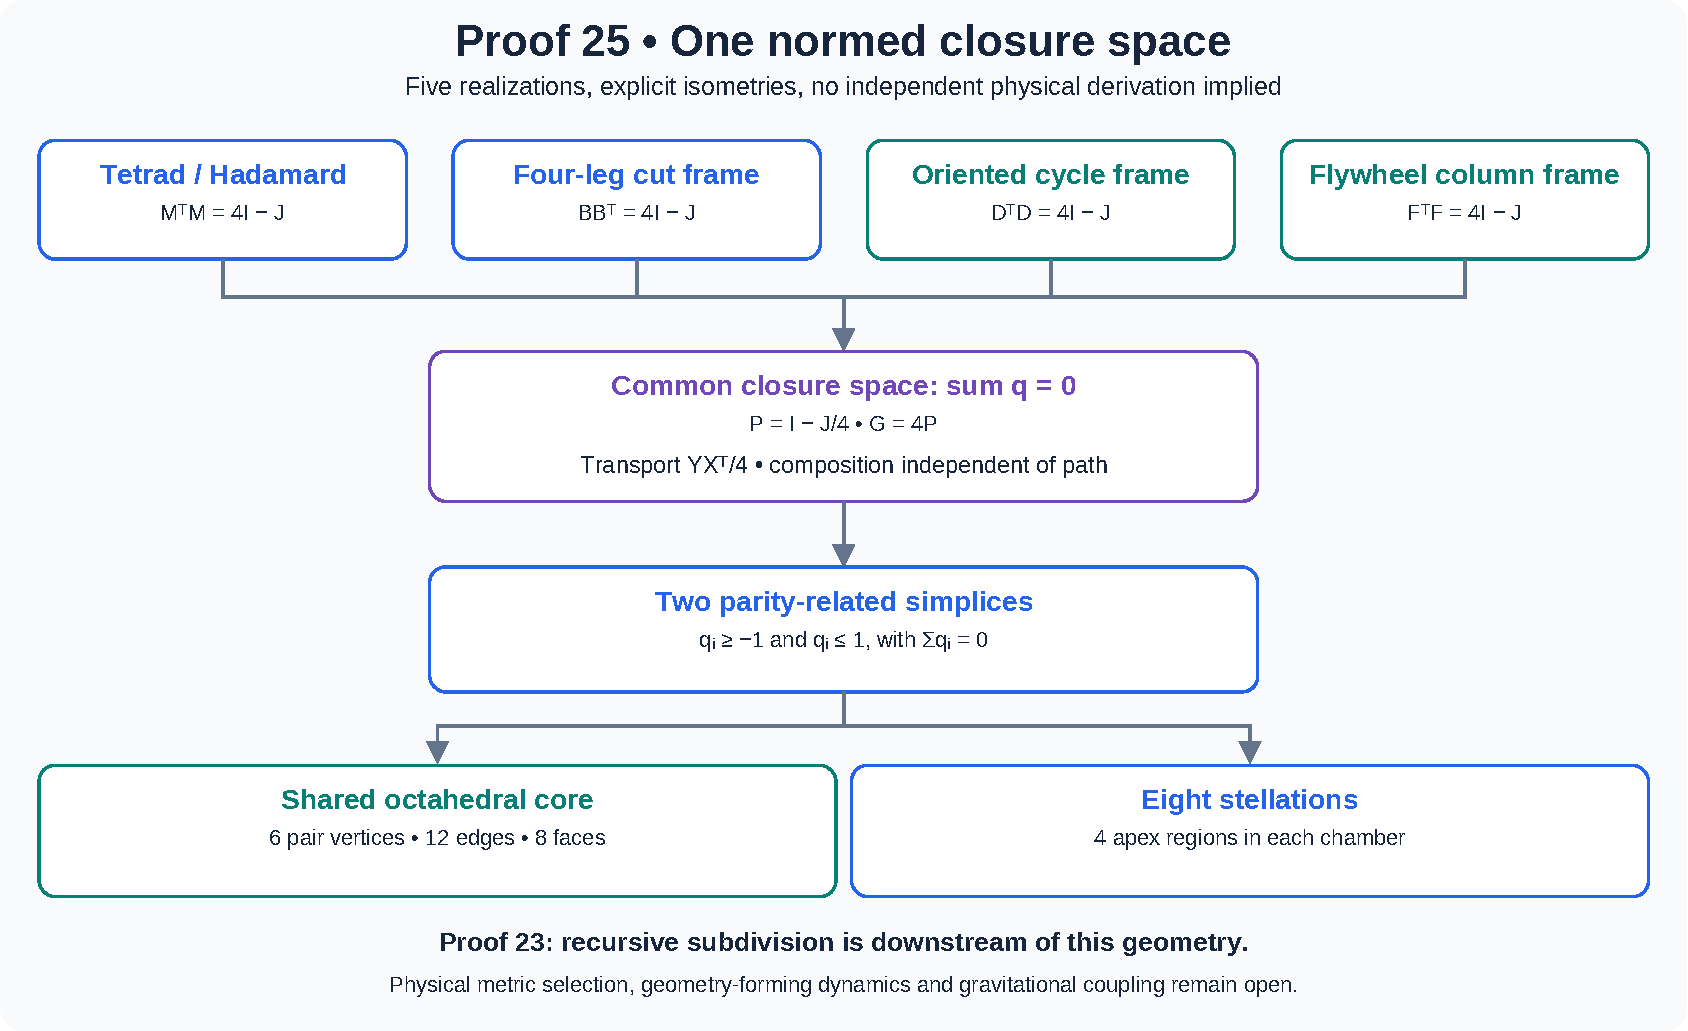
\includegraphics[width=.78\textwidth]{figures/convergence.pdf}
\end{center}
\noindent\textbf{Figure 1.} The four constructed frames and the intrinsic closure-space realization have one common normalized Gram; the maps of Theorem 3 link them without path dependence. The geometry follows after the stipulated metric and orientation assumptions.
\vspace{1mm}
\begin{center}
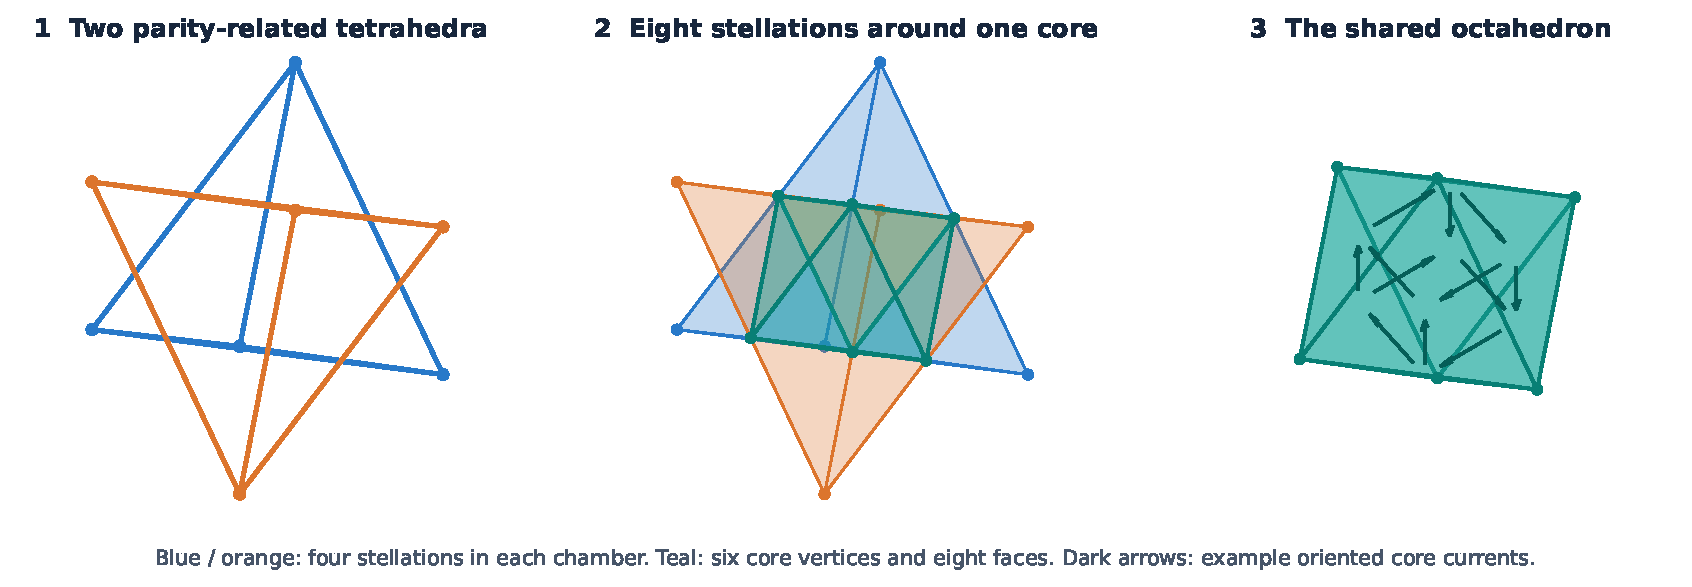
\includegraphics[width=.94\textwidth]{figures/stellations_and_core.pdf}
\end{center}
\noindent\textbf{Figure 2.} Exact three-dimensional coordinate rendering of the dual tetrahedra, eight actual stellations and shared core. Dark arrows illustrate the direction of an example Stage VII core current on the face-dual graph, not physical fluid streamlines or axial flow.
\vspace{1mm}
\begin{center}
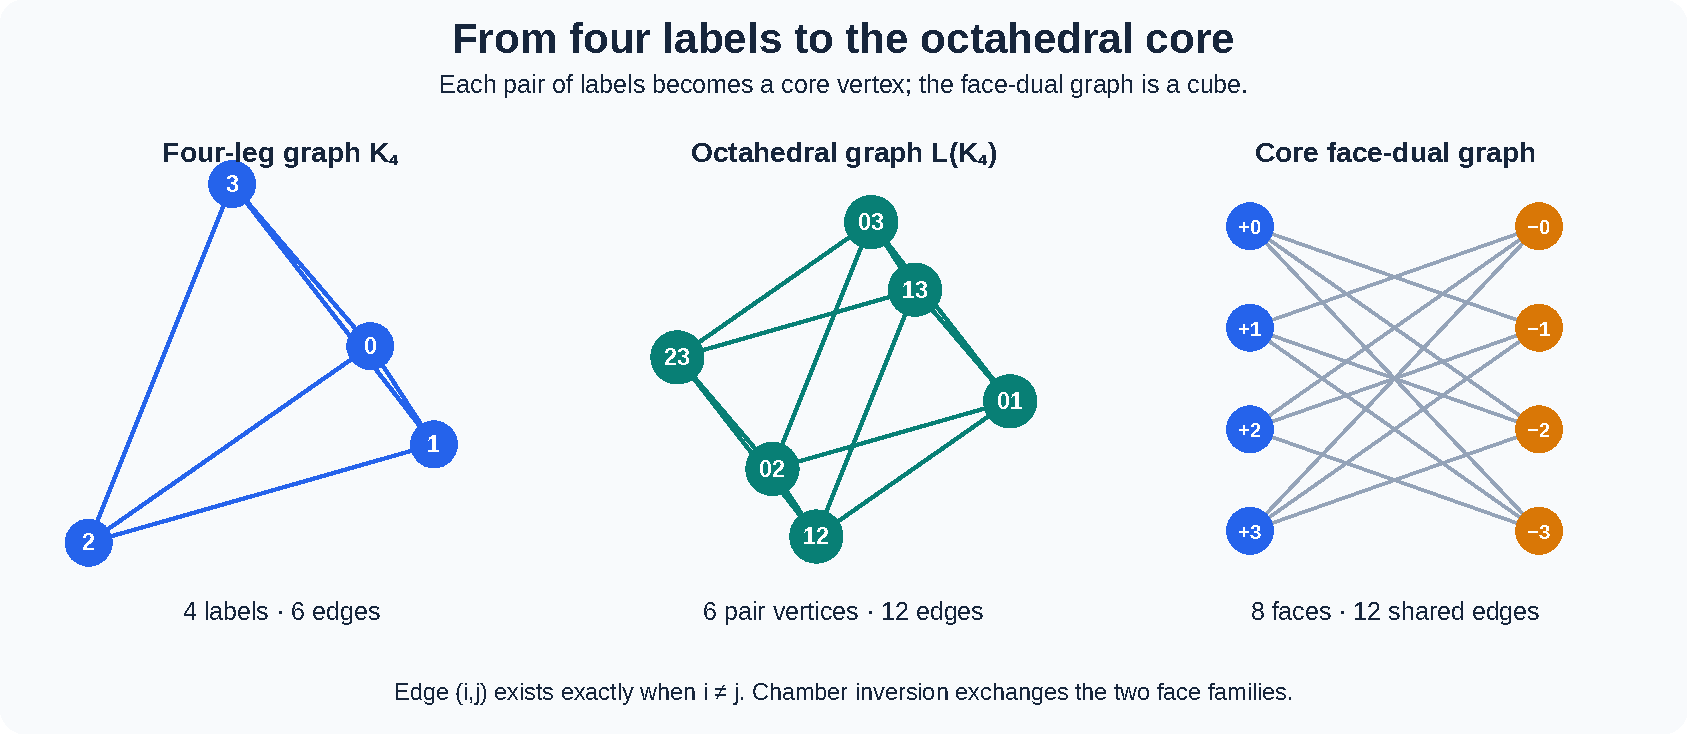
\includegraphics[width=.82\textwidth]{figures/core-incidence.pdf}
\end{center}
\noindent\textbf{Figure 3.} The pair incidence of $K_4$ produces the octahedral graph, and the octahedron's face-dual is the crown graph. Each dual edge corresponds to a single shared primal edge.
\end{document}
